\documentclass{article}

\usepackage{amsmath, amsfonts, amssymb}
\usepackage{fancyvrb}
\usepackage{graphicx}
\usepackage{multicol}

\title{Homework 7}
\author{Matthew Dupraz}

\begin{document}

\maketitle

\subsection*{(a)}


\begin{align*}
	(A + uv^T)&(A^{-1} - \frac{1}{1 + v^TA^{-1}u}A^{-1}uv^TA^{-1}) = \\
	&= I_n - \frac{uv^TA^{-1}}{1 + v^TA^{-1}u} + uv^TA^{-1}
	- \frac{(uv^TA^{-1})^2}{1+v^TA^{-1}u}\\
	&= I_n + uv^TA^{-1} - \frac{uv^TA^{-1} + uv^TA^{-1}uv^TA^{-1}}
	{1 + v^TA^{-1}u}\\
	&= I_n + uv^TA^{-1} - \frac{u(1 + v^TA^{-1}u)v^TA^{-1}}
	{1 + v^TA^{-1}u}\\
	&= I_n + uv^TA^{-1} - uv^TA^{-1} = I_n,
\end{align*}
and so this implies
\begin{equation*}
	(A + uv^T)^{-1} = A^{-1} - \frac{1}{1 + v^TA^{-1}u}A^{-1}uv^TA^{-1}
\end{equation*}

\subsection*{(b)}

Suppose $-1 = v^TA^{-1}u$ and ad absurdum suppose $A + uv^T$ is non-singular,
then
\begin{equation*}
	(A + uv^T)(A^{-1}u) = AA^{-1} + uv^TA^{-1}u = u - u = 0,
\end{equation*}
but $A^{-1}u$ is non-zero, since $v^TA^{-1}u = -1$, but this contradicts the
fact that $A + uv^T$ is non-singular.

\subsection*{(c)}
We have that $B$ is of the form $A + uv^T$, where for example
\begin{align*}
	u &= (1, 0, \dots, 0, 1)^T\\
	v &= (\beta_n, 0, \dots, 0, \beta_n)^T.
\end{align*}
It is easy to see then, that $A$ is tridiagonal, which means we can solve
equations of the form $Ax = b$ with linear complexity.

Now consider the problem $Bx = b$. This is equivalent to 
$(A + uv^T)x = b$ or also $x = (A + uv^T)^{-1}b$. So using the Sherman-Morisson
formula, we get
\begin{align*}
	x &= \left(A^{-1} - \frac{1}{1 + v^TA^{-1}u}A^{-1}uv^TA^{-1}\right)b\\
	&= A^{-1}b - \frac{1}{1 + v^TA^{-1}u}A^{-1}uv^TA^{-1}b
\end{align*}
Now we can compute $y = A^{-1}u$ and $z = A^{-1}b$ with linear complexity
(this is equivalent to solving $Ay = u$, resp. $Az = b$),
and so we get the formula
\begin{equation*}
	x = z - \frac{1}{v^Ty}yuv^Tz
\end{equation*}
So we can write the following algorithm for solving $Bx = b$ of complexity
$O(n)$:
\begin{enumerate}
	\item Solve $Ay = u$ for $u$.
	\item Solve $Az = b$ for $z$.
	\item $x \leftarrow z - \frac{1}{v^Ty}yuv^Tz$

\end{enumerate}

\subsection*{(d)}

I got the following values from running {\tt main.m}:
\begin{Verbatim}[frame=single,
	label=Output of main.m]
x = 
    5.0000
    1.0000
   -2.0000
   -4.0000
   -5.0000
   -5.0000
   -4.0000
   -2.0000
    1.0000
    5.0000

Relative error: 2.679297e-15
\end{Verbatim}

Graphing the time the algorithm took to finish against the size of the matrix
produced the following figure:
\begin{center}
	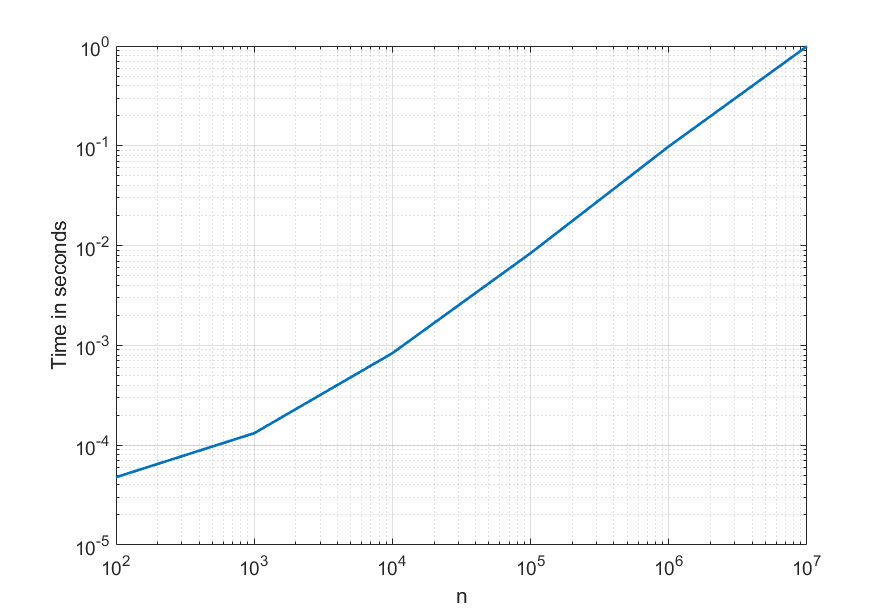
\includegraphics[scale=0.6]{figure.png}
\end{center}

Here follows the code used:
\begin{Verbatim}[frame=single,
	label=\textsc{Matlab} code - solve.m]
function [x, t, B, b] = solve(n)
    %Initialize matrix B
    A = sparse_matrix(n);
    u = sparse([1, n], [1, 1], [1, 1]);
    v = u;
    B = A + u*v';
    b = ones(n, 1);

    % We don't count initializing B towards the solving time
    tic;
    % Since A is tridiagonal, we can compute y and z
    % with linear complexity
    y = A\u;
    z = A\b;
    x = z - 1/(1 + v' * y) * y * v' * z;
    t = toc;
end
\end{Verbatim}

\begin{Verbatim}[frame=single,
	label=\textsc{Matlab} code - main.m]
% Solve for n=10 and display the relative error
[x, ~, B, b] = solve(10);
fprintf("x = \n")
disp(x');
error = norm(B*x - b)/norm(b);
fprintf("Relative error: %d\n", error);

% Solve for large n and measure the time taken
t = zeros(1, 6);
for i = 2:7
	[~, t(i-1)] = solve(10^i);
end

% Plot time taken against n
loglog(10.^(2:7), t);
ylabel('Time in seconds');
xlabel('n');
grid on;

\end{Verbatim}

\end{document}
